\documentclass[a4paper]{article}
\usepackage[english]{babel}
\usepackage[utf8]{inputenc}

%
% Graphics
%
\usepackage{graphicx}
\usepackage{xcolor}

\definecolor{alpha}{HTML}{3FA9F5}

%
% Bibliography
%
\usepackage[backend=bibtex,maxnames=5,sorting=none,url=false]{biblatex}
\usepackage{csquotes}

%
% Listings
%
\usepackage{listings}

\definecolor{background}{HTML}{FAFAFA}
\definecolor{sign}{HTML}{3FA9F5}

\lstdefinelanguage{fortune}{
  basicstyle=\ttfamily,
  basewidth={0.5em,0.5em},
  backgroundcolor=\color{background},
  literate=
   *{\%}{{{\color{alpha}{\%}}}}{1}
}

\lstdefinelanguage{shell}{
  basicstyle=\ttfamily,
  basewidth={0.5em,0.5em},
  backgroundcolor=\color{background},
  literate=
    [*]{\\\$}{{{\color{alpha}{\$}}}}{1}
       {Command>}{{{\color{alpha}{Command>}}}}{8}
       {ivan(0)>}{{{\color{alpha}{ivan(0)>}}}}{8}
       {ivan(1)>}{{{\color{alpha}{ivan(1)>}}}}{8}
       {ivan(0):RELEASED>}{{{\color{alpha}{ivan(0):RELEASED>}}}}{17}
       {ivan(0):LOCKED>}{{{\color{alpha}{ivan(0):LOCKED>}}}}{15}
       {ivan(1):LOCKED>}{{{\color{alpha}{ivan(1):LOCKED>}}}}{15}
       {ivan(2):LOCKED>}{{{\color{alpha}{ivan(2):LOCKED>}}}}{15}
}

\lstdefinelanguage{json}{
  basicstyle=\ttfamily,
  basewidth={0.5em,0.5em},
  backgroundcolor=\color{background},
  literate=
   *{:}{{{\color{alpha}{:}}}}{1}
    {,}{{{\color{alpha}{,}}}}{1}
    {\{}{{{\color{alpha}{\{}}}}{1}
    {\}}{{{\color{alpha}{\}}}}}{1}
    {[}{{{\color{alpha}{[}}}}{1}
    {]}{{{\color{alpha}{]}}}}{1}
}

\lstnewenvironment{fortune}%
{\lstset{language=fortune}}%
{}

\lstnewenvironment{json}%
{\lstset{language=json}}%
{}

\lstnewenvironment{shell}%
{\lstset{language=shell}}%
{}

%
% Links
%
\usepackage{hyperref}
\hypersetup{%
  colorlinks=true,
  citecolor={alpha},
  linkcolor={alpha},
  urlcolor ={alpha}
}

%
% Text
%
\newcommand{\ie}{i.e.}
\newcommand{\eg}{e.g.}
\newcommand{\etc}{etc.}

\newcommand{\fix}{should be modified}
\newcommand{\leave}{no changes are needed}
\newcommand{\overwrite}{should contain your previous changes}

\newcommand{\python}{\texttt{Python}}
\newcommand{\classname}[1]{\texttt{#1}}
\newcommand{\filename}[1]{\texttt{#1}}
\newcommand{\code}[1]{\texttt{#1}}

%
% References
%
\newcommand{\sref}[1]{Section~\ref{sec:#1}}
\newcommand{\tref}[1]{Table~\ref{tab:#1}}
\newcommand{\fref}[1]{Figure~\ref{fig:#1}}

\newcommand{\slabel}[1]{\label{sec:#1}}
\newcommand{\tlabel}[1]{\label{tab:#1}}
\newcommand{\flabel}[1]{\label{fig:#1}}

\newcommand{\slab}[1]{\label{sec:#1}}
\newcommand{\tlab}[1]{\label{tab:#1}}
\newcommand{\flab}[1]{\label{fig:#1}}

\newcommand{\aref}[1]{Lab~#1 \cite{description#1}}


\bibliography{include/references.bib}

\title{%
  Distributed Systems: Lab 1\\%
  Client-Server Database%
}
\author{Petru Eles, Adrian Horga, and Ivan Ukhov\\
\vspace{0.5em}
\href{mailto:petru.eles@liu.se}{petru.eles@liu.se},
\href{mailto:petru.eles@liu.se}{adrian.horga@liu.se}, and
\href{mailto:ivan.ukhov@liu.se}{ivan.ukhov@liu.se}
}
\date{December 27, 2016}

\begin{document}
\maketitle

\section{Introduction}
\begin{figure}
  \centering
  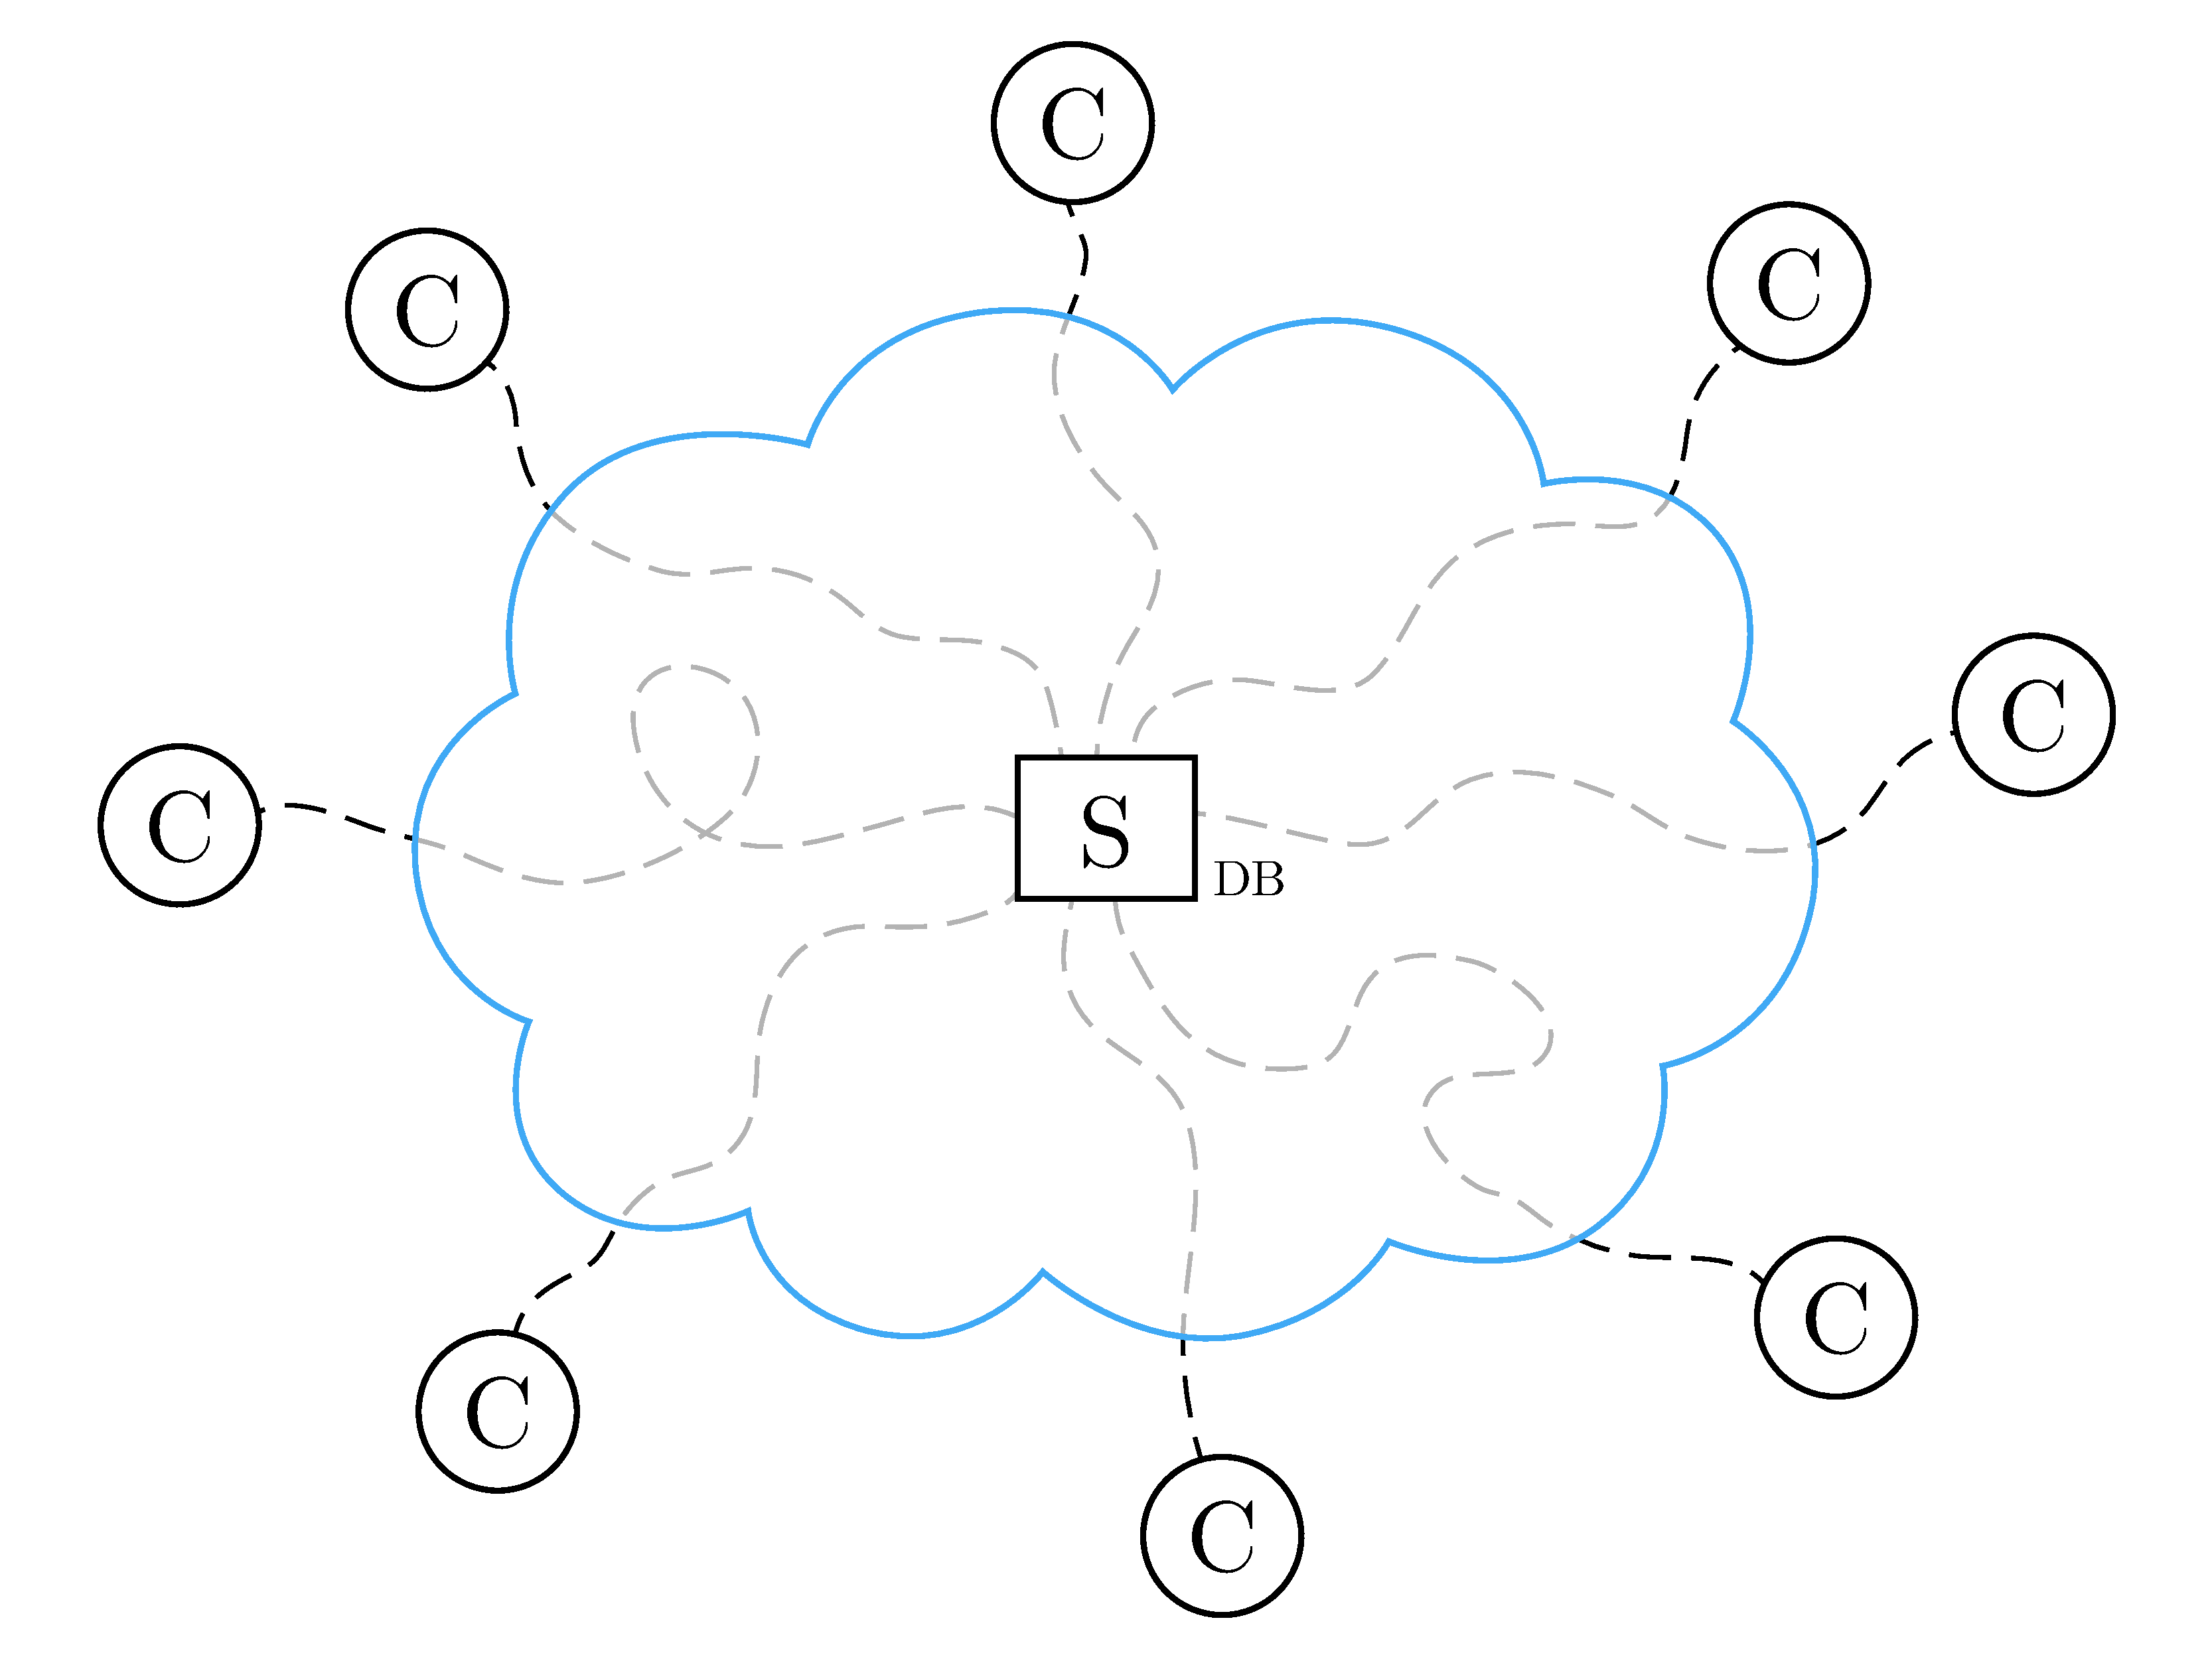
\includegraphics[width=0.8\textwidth]{include/assets/single-server.pdf}
  \caption{A distributed database with a single server (S), maintaining a database (DB), and a number of clients (C).}
  \flabel{single-server}
\end{figure}

In the previous lab, you built a non-distributed system composed of a number of
standalone machines, and each such machine was responsible for both the server
and client components of your fortune database. You observed that the private
copies of the data maintained by the machines could easily become inconsistent
as there were no attempts of synchronization. The goal of the current lab is to
mitigate this problem by utilizing the client-server model \cite{lecture2} of
distributed systems. Specifically, we shall designate the server role to one
separate machine and turn the rest into pure clients. This scenario is depicted
in \fref{single-server}; compare it with the one from \aref{0}.

\section{Communication Protocol} \slab{protocol}
In order for the server and clients to be able to interact with each other, they
need to agree upon a communication protocol. In this programming project, the
communication protocol has the following specification.

Each message is encoded in the JSON format \cite{json, python-json} and sent as
a single line, which ends with a new-line character. Whenever a client wants to
invoke a function on the server side, the client sends a message to the server
using the following scheme:
\begin{json}
{
    "method": method_name,
    "args": method_arguments
}
\end{json}
The \texttt{method} field contains a string with the name of the function that
the client wants to call, and the \texttt{args} field contains an array of
arguments that that function takes. For example, in order to add a new fortune
into the database of the server, a client might send the following message:
\begin{json}
{
    "method": "write",
    "args": ["Take it easy"]
}
\end{json}
meaning that the method to invoke is called ``write,'' and ``Take it easy''
should be passed as the first and the only argument of that method. As noted
earlier, it is important to send each message as a single line terminated by a
new-line character; make sure you follow this convention when writing into the
socket.

If a method invocation is successful, the server sends an acknowledgment to the
corresponding client using the following scheme:
\begin{json}
{
    "result": method_result
}
\end{json}
where the \texttt{result} field contains the output of the executed function
encoded in the JSON format; the whole message is a single line. Note that the
presence of this field is sufficient to conclude that the call was successful,
and the value of the field can be \code{null} if the corresponding function
returns nothing.

If a method invocation fails due to an error, the server replies with a message
having the following structure:
\begin{json}
{
    "error": {
        "name": error_class_name,
        "args": error_arguments
    }
}
\end{json}
The occurred error is encoded in \texttt{error} in such a way that it can be
instantiated and raised on the client side; in fact, it is one of the
requirements to your implementation. At this point, it is worth recalling that
an exception in \python\ is an instance of some exception class. In order to
create such an instance, one has to know the name of the exception class and the
arguments that the class' constructor requires. With this in mind, the
\texttt{name} field delivers the class name of the occurred exception while
\texttt{args} delivers an array of the parameters to be passed to the
constructor of the class.

\section{Your Task}
\subsection{Preparation}
Continue working with the same code base that you have been working with so far,
including all the changes that you have made. The files relevant to this lab are
listed below. You should read and understand them.
\begin{itemize}

  \item \filename{lab1/client.py} --- the \classname{Client} application (\fix);

  \item \filename{lab1/server.py} --- the \classname{Server} application (\fix);

  \item \filename{lab1/test.sh} --- a shell script that you can use for testing;

  \item \filename{lab1/dbs/fortune.db} --- the same as for \aref{0};

  \item \filename{modules/Common/wrap.sh} --- an auxiliary script needed for
  \filename{test.sh};

  \item \filename{modules/Server/lock/readWriteLock.py} --- the class utilized
  by \classname{Server} for the purpose of synchronization as motivated in
  \sref{communication} (\leave);

  \item \filename{modules/Server/database.py} --- the same as for \aref{0}
  (\overwrite).

\end{itemize}
Carefully read the source code and understand what it is doing. Pay your
attention to the missing parts marked with ``Your code here.'' In order to run
the code, open two terminal windows and change the current folder to
\filename{lab1}. In one of the terminals, issue the following command in order
to run the \classname{Server} application (recall that the server is unique in
this lab):
\begin{shell}
\$ ./server.py
Listening to: c-204-13.eduroam.liu.se:45725
Press Ctrl-C to stop the server...
\end{shell}
The code randomly chooses a port number to listen to and prints it out along
with the hostname of the server machine. In the example given above, the
hostname is \texttt{c-204-13.eduroam.liu.se}, and the port number is
\texttt{45725}. As you have already discovered by studying the code in
\filename{server.py}, you can choose a port number yourself by specifying the
corresponding argument in the command line. Now, let us create an instance of
the \classname{Client} application by running the following command in the
second terminal:
\begin{shell}
\$ ./client.py -i c-204-13.eduroam.liu.se:45725
Choose one of the following commands:
    r            ::  read a random fortune from the database,
    w <FORTUNE>  ::  write a new fortune into the database,
    h            ::  print this menu,
    q            ::  exit the application.

Command> w Keep it simple.
Command> r
None
Command>
\end{shell}
Note that you have to specify the address that your server is using, and it can
be a different address each time you restart the server. Regardless of the
correctness of the address, the system does not work at this stage since neither
\classname{Server} nor \classname{Client} has the corresponding communication
part implemented.

In order to ease the testing procedure of this and the future labs, we have
implemented a set of shell scripts that open the needed terminals and run the
corresponding commands for you. These scripts are called \filename{test.sh} and
can be found in the main folder of each lab. For instance, the test script for
the current lab is \filename{lab1/test.sh}. It is important to note, however,
that you should be able to set up everything yourself without the help of these
scripts. So, have a look at the content of the scripts and make sure you
understand what they do. You can also modify these scripts as you wish.

\subsection{Communication} \slab{communication}
Using \python's sockets \cite{python-ipc}, complete the implementation of
\filename{server.py} and \filename{client.py}. Your code should satisfy the
following requirements:
\begin{itemize}

  \item Both \classname{Server} and \classname{Client} should implement and
  follow the communication protocol described in \sref{protocol}.

  \item The server should process each client in a separate thread such that it
  does not stop serving other incoming connections. Your implementation should
  be thread safe as motivated below.

  \item The server should be robust: it should catch and adequately respond to
  exceptions including those due to potential network problems, violations of
  the protocol, invocations of non-existing functions, invocations of proper
  functions but with wrong arguments, \etc

  \item Whenever a client receives an error from the server, it should
  instantiate and raise it as if the error has occurred locally. The user of the
  \classname{Client} application should not feel any difference between the
  non-distributed and distributed versions of the system.

\end{itemize}

Since the server can have several threads serving client requests in parallel,
the operations on the database issued by the clients can interfere with each
other and leave the database in a corrupted state. In order to prevent this
behavior, you should protect the critical parts of your code with a read/write
lock provided to you in \filename{readWriteLock.py}. Think where the locking
should take place and how to make it efficient in terms of the waiting time.

Lastly, make sure that, in spite of all possibly occurred exceptions, the server
keeps on working until it is explicitly stopped by the user.

\section{Conclusion}
In this lab, you have implemented a rather na\"{i}ve distributed system: there
is only one server and each client is required to know the current address of
the server. The former issue makes our distributed system both unreliable (\eg,
your carefully written code will not protect the server against a blackout) and
inefficient (\eg, if there are many clients, the workload of a single server
machine can be substantially high making clients wait for a response for a long
time). The second issue makes it inconvenient for the clients to connect to the
server as the hostname and/or port of the server might easily change, and the
clients need to keep track of such changes. This inconvenience will become
especially bothering when you allow your distributed system to have several
servers; therefore, in the next lab, you will address this problem first.

\printbibliography

\end{document}
